\documentclass[11pt,a4paper]{article}
\usepackage[utf8]{inputenc}
\usepackage[T1]{fontenc}
\usepackage{amsfonts}
\usepackage[francais]{babel}
\usepackage{enumitem}
\usepackage{amssymb}
\usepackage{amsmath}
\usepackage[left=2cm,right=2cm,top=2cm,bottom=2cm]{geometry}
\usepackage{multirow}
\usepackage[dvipsnames]{xcolor}
\usepackage{graphicx}
\usepackage{setspace}
\singlespacing
\usepackage{tikz}
\usetikzlibrary{arrows.meta}

\usepackage{multicol}
\usepackage{caption}
\usepackage{fancyhdr}
\pagestyle{fancy}
\renewcommand\headrulewidth{1pt}
\fancyhead[L]{Lycée Denis Diderot }
\fancyhead[R]{Classe de Terminale -- \textcolor{red}{\textbf{CORRIGÉ}}}
\setcounter{page}{6}\fancyfoot[C]{page \thepage}
\fancyfoot[R]{Année 2025 2026}
\fancyfoot[L]{Alexis RUIZ}
\usepackage{multirow,tabularx,booktabs}
\newcommand{\cadreblanc}[1]{%
\medskip\framebox[\linewidth][c]{%
\rule{0mm}{#1mm}}\par
\medskip}

% Commandes simplifiées pour remplacer les packages manquants
\newcommand{\ch}[1]{\textrm{#1}}
\newcommand{\pch}[1][]{$^{#1+}$}
\newcommand{\ecrire}[1]{#1}

\renewcommand{\arraystretch}{2}
\newcommand*\acocher{\quitvmode{\fboxsep0pt \fboxrule0.8pt \fbox{\vrule height1.8ex depth.1ex width0pt \vrule height0pt depth0pt width1.9ex }}}

\begin{document}




\section*{I - Couple redox}

\ecrire{\fbox{
\begin{minipage}{14cm}{
\textcolor{red}{\textbf{Définition :}} \\
\textcolor{red}{Un \textbf{couple redox} (ou couple oxydant/réducteur) est constitué d'un \textbf{oxydant} et de son \textbf{réducteur conjugué}.}\\[0.3cm]
\textcolor{red}{On note un couple redox : \textbf{Oxydant / Réducteur} ou \textbf{Ox/Red}}\\[0.3cm]
\textcolor{red}{\textbf{Exemples :}}\\
\textcolor{red}{$\bullet$ Le couple \ch{Cu}$^{2+}$/Cu : l'ion cuivre II \ch{Cu}$^{2+}$ est l'oxydant et le cuivre Cu est le réducteur.}\\
\textcolor{red}{$\bullet$ Le couple \ch{Fe}$^{2+}$/Fe : l'ion fer II \ch{Fe}$^{2+}$ est l'oxydant et le fer Fe est le réducteur.}\\[0.3cm]
\textcolor{red}{\textbf{Demi-équation électronique :}}\\
\textcolor{red}{La transformation d'un oxydant en réducteur (ou inversement) fait intervenir un \textbf{échange d'électrons}.}\\
\textcolor{red}{On écrit : \fbox{Oxydant + n e\textsuperscript{-} $\rightleftharpoons$ Réducteur}}\\[0.2cm]
\textcolor{red}{Exemple : \ch{Cu}$^{2+}$ + 2 e\textsuperscript{-} $\rightleftharpoons$ Cu}\\
}

\end{minipage}
}}
\vspace {0.5cm}

\section*{II - Classification}

Les couples redox sont classées d'après leur pouvoir oxydant ( et donc réducteur aussi ) dans la classification électrochimique des métaux ci-dessous.

\begin{center}
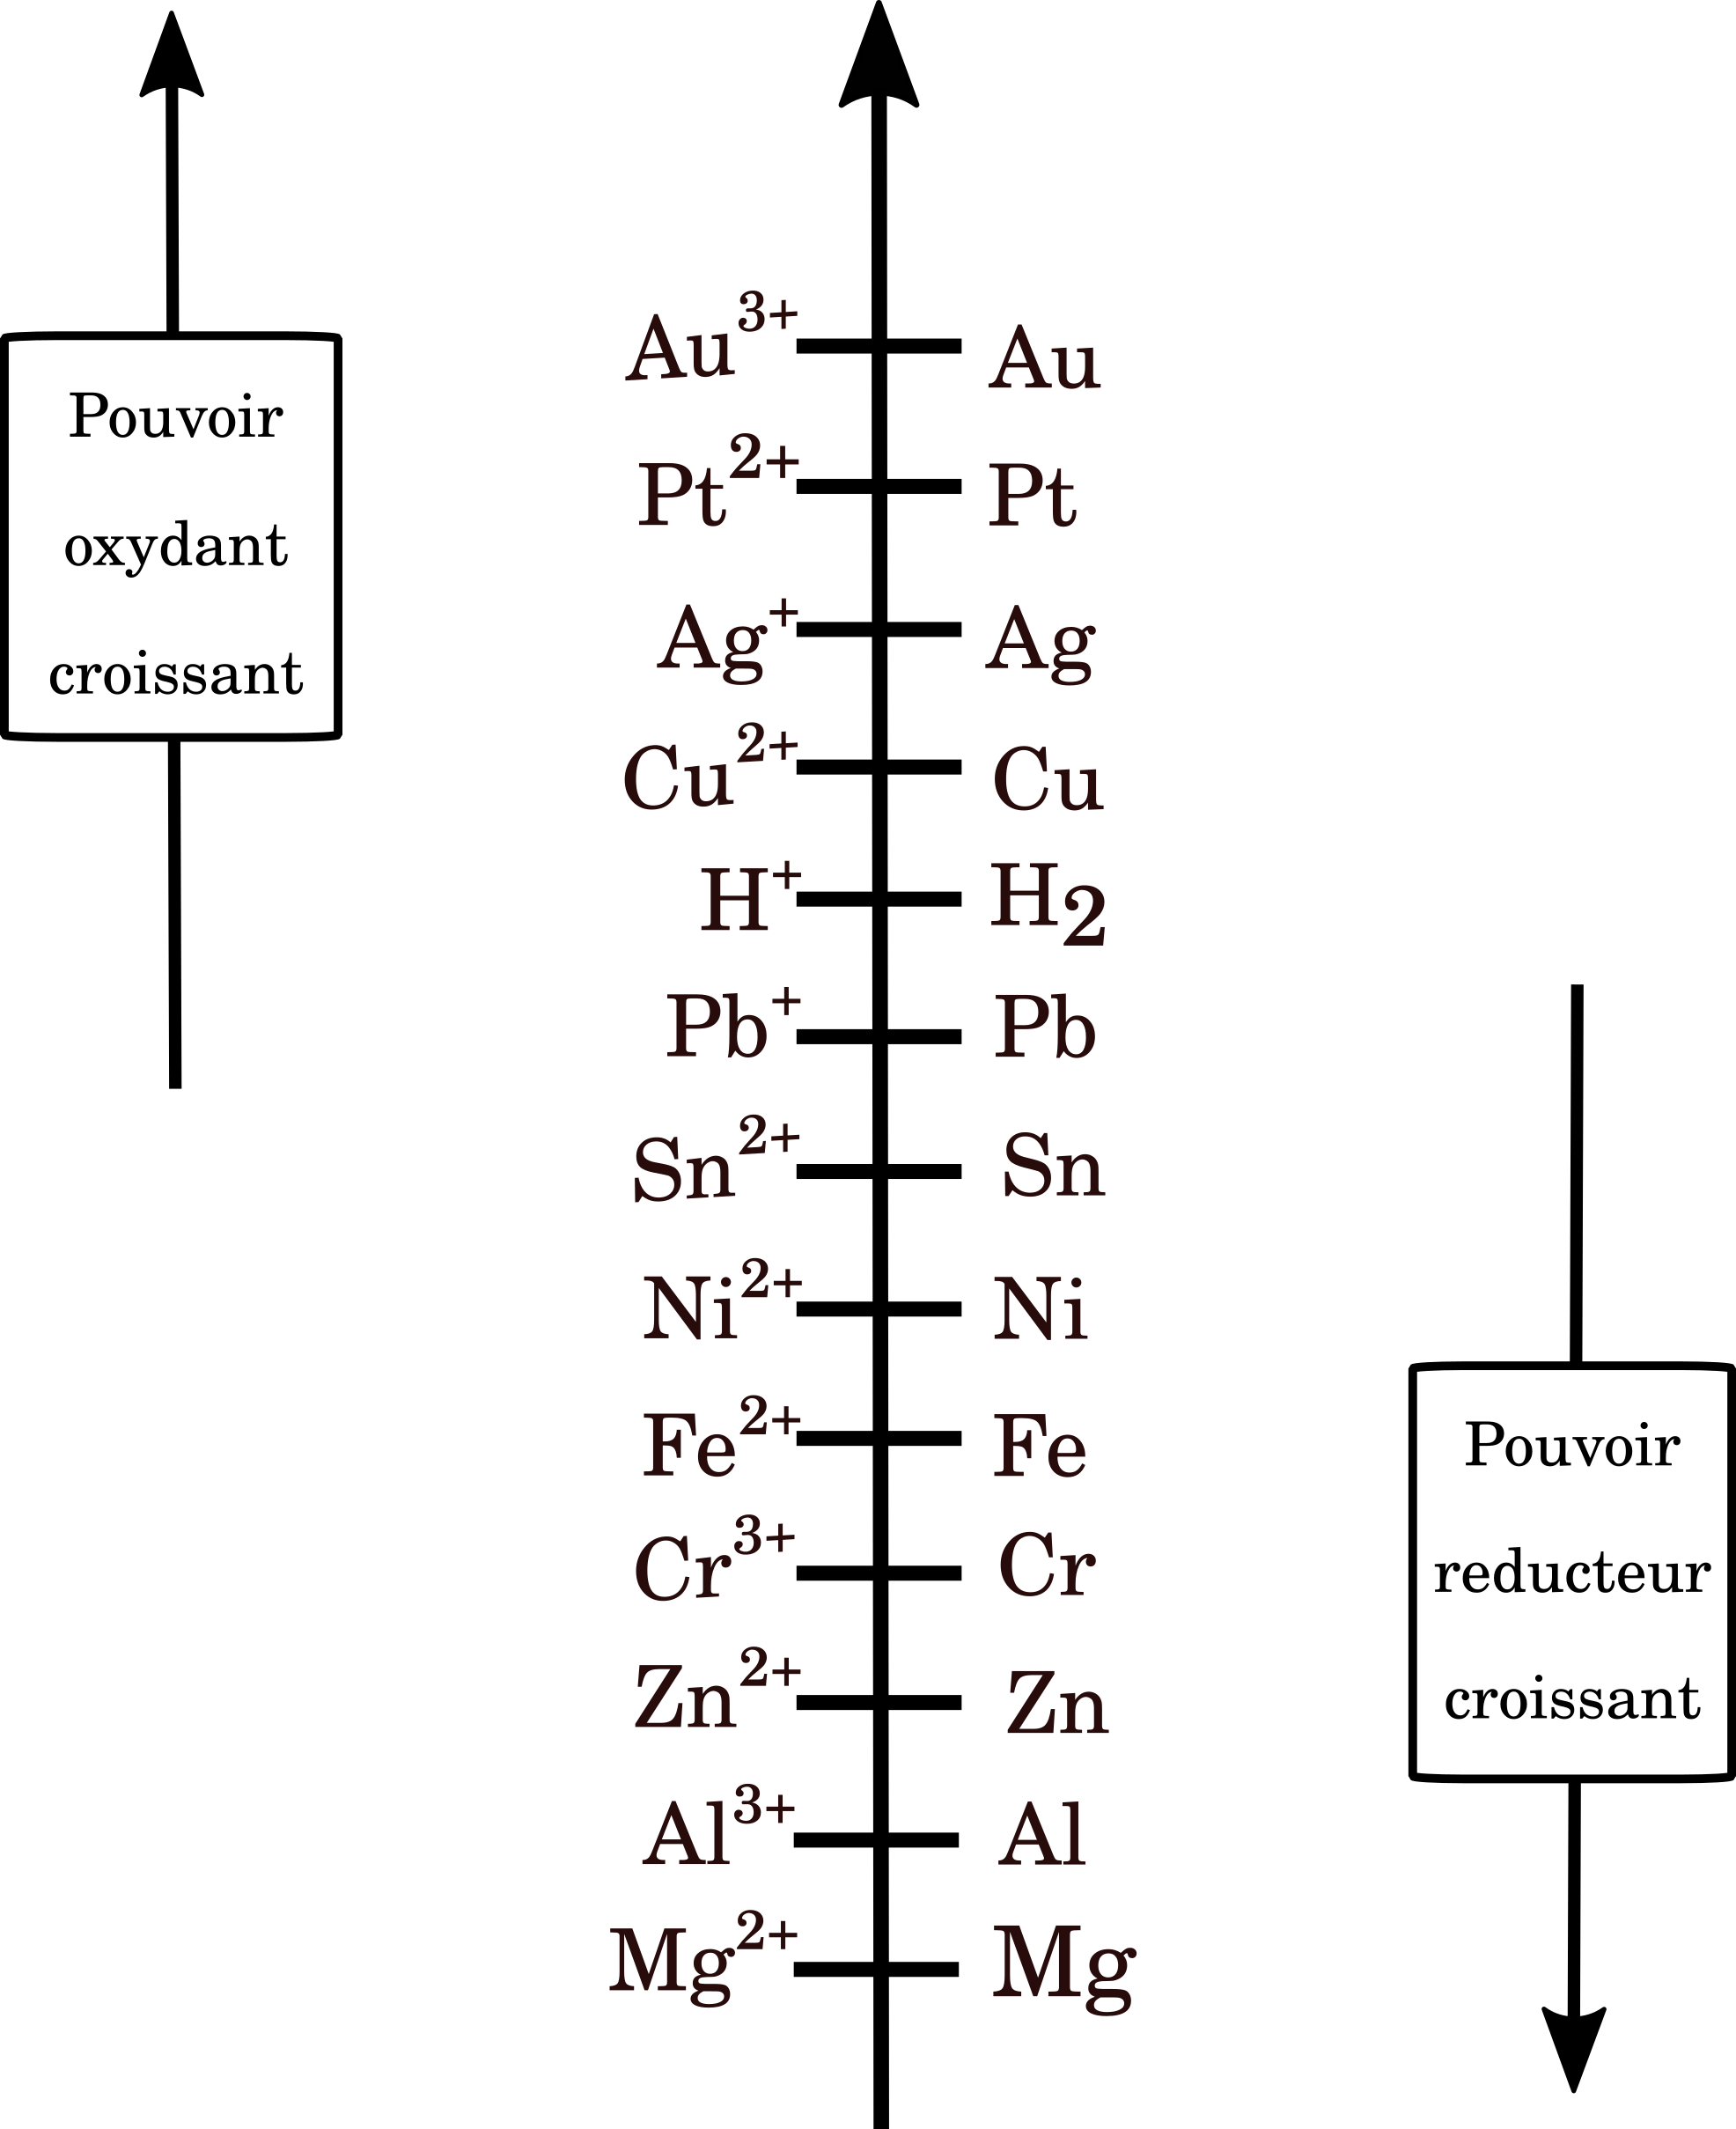
\includegraphics[scale=0.3]{images/classification.png}
\end{center}

\vspace {0.5cm}

\section*{III - Règle du gamma}
\begin{itemize}
\item Elle permet d'expliquer pourquoi la réaction d'oxydoréduction se réalise dans le cas d'une lame de fer dans des ions \ch{Cu}$^{2+}$ et ne se réalise pas dans le cas d'une lame de Cu dans des ions \ch{Fe}$^{2+}$. 
\item Elle est un moyen rapide pour savoir quelle réaction se produit spontanément.
\end{itemize}


\textbf{Exemple :} On trempe une lame de zinc (Zn) dans une solution contenant des ions argent (\ch{Ag}$^{+}$)



\begin{figure}[h]
\begin{minipage}{0.45\textwidth}
\begin{center}
\begin{tikzpicture}[scale=1.4]
% Échelle verticale noire
\draw[thick, black] (0,0) -- (0,4.5);

% Positions des couples - disposition en croix
% Ag+ et Ag en haut
\node at (-1.2, 3.5) {\ch{Ag}$^{+}$};
\node at (1.2, 3.5) {Ag};
% Zn^2+ et Zn en bas
\node at (-1.2, 1) {\ch{Zn}$^{2+}$};
\node at (1.2, 1) {Zn};

% Labels
\node[font=\scriptsize, align=center] at (-1.8,3.5) {Oxydant\\le plus\\fort};
\node[font=\scriptsize, align=center] at (1.8,1) {Réducteur\\le plus\\fort};

% Gamma avec parcours complet et flèches
% 1. De Ag+ vers Zn (descente à droite)
\draw[-latex, green!60!black, line width=2.5pt] (-1.2, 3.3) -- (1.0, 1.2);

% 2. De Zn vers Zn^2+ (horizontale vers la gauche)
\draw[-latex, blue, line width=2.5pt] (1.0, 1) -- (-1.0, 1);

% 3. De Zn^2+ remonte vers Ag (remontée à droite)
\draw[-latex, red!70!black, line width=2.5pt] (-1.2, 1.2) -- (1.0, 3.3);

% Texte réaction
\node[red, font=\small\bfseries] at (0,-0.3) {réaction spontanée};

% Légendes
\node[green!60!black, font=\tiny, align=left] at (0.8, 2.5) {réduction\\Ag$^+$ + e$^-$};
\node[blue, font=\tiny, align=left] at (0, 0.5) {oxydation : Zn $\rightarrow$ Zn$^{2+}$ + 2e$^-$};
\end{tikzpicture}
\end{center}
\end{minipage}%
\begin{minipage}{0.55\textwidth}
1. En utilisant la classification (page~~6) placer les couples redox \ch{Ag}$^{+}$/ Ag et \ch{Zn}$^{2+}$/Zn. \\

\textcolor{red}{Voir schéma ci-contre.}\\

2. Tracer sur l'échelle le gamma. \\

\textcolor{red}{Voir schéma ci-contre.}\\

\end{minipage}
\end{figure}
3. La réaction peut – elle avoir lieu ?\\

\textcolor{red}{Oui, la réaction peut avoir lieu car le gamma pointe vers le haut.}\\

4. Écrire les deux demi équations correspondantes à cette réaction. \\
\begin{center}
\fbox{\textcolor{red}{$\ch{Zn}$ $\longrightarrow$ \ch{Zn}$^{2+}$ + 2 e\textsuperscript{-}}}\\[3mm]
\fbox{\textcolor{red}{\ch{Ag}$^{+}$ + e\textsuperscript{-} $\longrightarrow$ \ch{Ag}}}\\
\end{center}
\normalsize
5. Écrire l'équation de la réaction. \\
\begin{center}
\fbox{\textcolor{red}{\ch{Zn} + 2 \ch{Ag}$^{+}$ $\longrightarrow$ \ch{Zn}$^{2+}$ + 2 \ch{Ag}}}\\
\end{center}

\textbf{Exercice :} On trempe une bague en argent (Ag) dans une solution contenant des ions or (\ch{Au}$^{3+}$)



\begin{figure}[h]
\begin{minipage}{0.45\textwidth}
\begin{center}
\begin{tikzpicture}[scale=1.4]
% Échelle verticale noire
\draw[thick, black] (0,0) -- (0,4.5);

% Positions des couples - disposition en croix
% Au^3+ et Au en haut
\node at (-1.2, 3.5) {\ch{Au}$^{3+}$};
\node at (1.2, 3.5) {Au};
% Ag+ et Ag en bas
\node at (-1.2, 1.2) {\ch{Ag}$^{+}$};
\node at (1.2, 1.2) {Ag};

% Labels
\node[font=\scriptsize, align=center] at (-1.8,3.5) {Oxydant\\le plus\\fort};
\node[font=\scriptsize, align=center] at (1.8,1.2) {Réducteur\\le plus\\fort};

% Gamma avec parcours complet et flèches
% 1. De Au^3+ vers Ag (descente à droite)
\draw[-latex, green!60!black, line width=2.5pt] (-1.2, 3.3) -- (1.0, 1.4);

% 2. De Ag vers Ag+ (horizontale vers la gauche)
\draw[-latex, blue, line width=2.5pt] (1.0, 1.2) -- (-1.0, 1.2);

% 3. De Ag+ remonte vers Au (remontée à droite)
\draw[-latex, red!70!black, line width=2.5pt] (-1.2, 1.4) -- (1.0, 3.3);

% Texte réaction
\node[red, font=\small\bfseries] at (0,-0.2) {réaction spontanée};

% Légendes
\node[green!60!black, font=\tiny, align=left] at (0.8, 2.6) {réduction\\Au$^{3+}$ + 3e$^-$};
\node[blue, font=\tiny, align=left] at (0, 0.7) {oxydation : Ag $\rightarrow$ Ag$^{+}$ + e$^-$};
\end{tikzpicture}
\end{center}
\end{minipage}%
\begin{minipage}{0.55\textwidth}
1. En utilisant la classification (page~~6) placer les couples redox \ch{Ag}$^{+}$/ Ag et \ch{Au}$^{3+}$/Au. \\

\textcolor{red}{Voir schéma ci-contre.}\\

2. Tracer sur l'échelle le gamma. \\

\textcolor{red}{Voir schéma ci-contre.}\\

\end{minipage}
\end{figure}
3. La réaction peut – elle avoir lieu ?\\

\textcolor{red}{Oui, la réaction peut avoir lieu car le gamma pointe vers le haut.}\\

4. Écrire les deux demi équations correspondantes à cette réaction. \\
\begin{center}
\fbox{\textcolor{red}{\ch{Ag} $\longrightarrow$ \ch{Ag}$^{+}$ + e\textsuperscript{-}}}\\[3mm]
\fbox{\textcolor{red}{\ch{Au}$^{3+}$ + 3 e\textsuperscript{-} $\longrightarrow$ \ch{Au}}}\\
\end{center}
\normalsize
5. Écrire l'équation de la réaction. \\
\begin{center}
\fbox{\textcolor{red}{3 \ch{Ag} + \ch{Au}$^{3+}$ $\longrightarrow$ 3 \ch{Ag}$^{+}$ + \ch{Au}}}\\
\end{center}
\end{document}